\documentclass[12pt,a4paper]{article}

%\usepackage{sbc-template}
\usepackage{graphicx,url}
\usepackage{siunitx}
\usepackage{indentfirst}
\usepackage[utf8]{inputenc}
\usepackage[portuguese]{babel}
\usepackage{amsmath}
\usepackage{amsfonts}
\usepackage{amssymb}
\usepackage{algorithmic	}

\def\s{\STATE}
\def\cc{\COMMENT}
\def\a{\alpha}
\def\dt{\Delta t}
\def\tt{\theta}

\usepackage[brazil]{babel}   
\usepackage[utf8]{inputenc}  
\usepackage[T1]{fontenc}
     
%\sloppy

\title{Difusão de calor bidimensional utilizando método de diferençãs finitas implícito e explícito}

\author{Samuel E. de A. Júnior\inst{1} \\Ricardo Reis Pereira\inst{1} Antônio Joel R. de Castro\inst{1}}

\address{Universidade Federal do Ceará(UFC) - Campus Quixadá\\
CEP 63902-580 – Quixadá – CE – Brasil
\email{\{ricardoreispereira, samuelevangelista.ti\}@gmail.com}
\email{joelcastro@fisica.ufc.br}
}

\begin{document} 

\maketitle

\begin{abstract}{
    This work was conducted with the objective of reviewing the results of studies in the area of pure diffusion and finite differences, as well as solving an inquiry reported by the author of the book \cite{boldrini1986algebra}. In order to apply the practical concepts in computation, differential equations and linear algebra, the work was implemented in C++ for better visualization of results and in order to confirm the results, an application that once abstracted, now becomes much more intuitive and visible with the results and tests. Some applications of numerical methods can be found in the middle of the article, as well as resolutions using explicit and implicit methods.
  }
  
  \textbf{Keywords:} Implicit, Explicit, Finite Differences.
\end{abstract}
     
\begin{resumo}{
    Este trabalho tem por objetivo revisar resultados de alguns estudos feitos sobre difusão de calor aplicando o método das diferenças finitas (Euler, Crank-Nicolsom e ADI). Foi  solucionado do problema apresentado o problema apresentado em  \cite{boldrini1986algebra} referente ao aquecimento de uma placa através dos bordos (condições de Dirichlet). O trabalho, de natueza numérica, visa utilizr cnnhecimetos nas áreas de equações diferenciais, álgebra linear e computalção.         
  }
  
  \textbf{Palavras-Chave:} Implícito, Explícito, Diferenças Finitas.
\end{resumo}

\section{Introdução} 

No âmbito físico, o estudo da transferência de calor ou difusão de calor, se dá pela transferência de energia térmica entre os átomos e suas moléculas vizinhas em um meio devido ao gradiente de temperatura. Este trabalho foi construído com o intuito de realizar uma revisão dos trabalhos existentes em relação a difusão de calor e também solucionar uma indagação deixada pelo autor do livro \cite{boldrini1986algebra}, na qual é solicitada a temperatura dos bordos de uma placa após seu equilíbrio térmico dado as condições de contorno. Foi solucionado uma equação diferencial conhecida como problema de laplace ou problema de fourier, aplicando a transferência de calor em uma placa com condições de Dirichlet. O método utilizado para solucionar a equação diferencial dada, foi o método das diferenças finitas que é um método utilizado para aproximar equações diferenciais parciais e ordinárias. Para fazer tal aproximação é necessário discretizar o domínio do problema abordado em uma malha.

A equação diferencial, dada pelo livro, que reage ao fluxo de calor:
\newline

\begin{enumerate}(I)
    \centering
    \item 
    \begin{eq}
        \fbox{\scalebox{1.0}{$\frac{\partial T}{\partial t} = c(\frac{\partial^2 T}{\partial x^2} + \frac{\partial^2 T}{\partial y^2})$}}
    \end{eq}
\end{enumerate}

\newline

Na equação (I) temos a constante $c$, que descreve a constante característica do material e a variação da temperatura no domínio bidimensional. Adiante serão demonstradas as resoluções aproximadas utilizando os métodos explicíto e implicíto no regime permanente.

\section{Aplicações} \label{sec:firstpage}
\subsection{Método matematicamente explícito e permanente}

Nesta sessão será apresentada a resolução da solução utilizando o método explicíto, que calcula o estado do sistema em um tempo posterior ao estado atual do sistema. Vamos ter como as interações atuais as que estão no período de $k$, e as posteriores as que estão no período de $k+1$. Se diz regime permanente porque no equilibŕio terminco, a variação do tempo é igual a 0, logo $\frac{\partial T}{\partial t} = 0$, como o material da placa é homogêneo vamos desconsiderar a variável característica do material. Com isso, temos a seguinte equação diferencial:

\newline

\begin{enumerate}(II)
    \centering
    \item 
    \begin{eq}
        \fbox{\scalebox{1.0}{$(\frac{\partial^2 T}{\partial x^2} + \frac{\partial^2 T}{\partial y^2}) = 0$}}
    \end{eq}
\end{enumerate}

\newline

Para resolvermos o problema com metódo da diferenças finitas vamos nos basear no artigo do \cite{R.R.Pereira}, a primorde temos que considerar a placa como uma malha para fazermos uma "aproximação discreta". A partir disso fazemos as seguintes operações para descretizar a equação e aproximar os resultado:

\newline
\newline

$(\frac{\partial^2 T}{\partial x^2})$\Big|_{(i, j)} \approx  $ T^{k}_{i+1, j} - 2T^{k+1}_{i, j} + T^{k}_{i-1, j}$

\newline


$(\frac{\partial^2 T}{\partial y^2})$\Big|_{(i, j)} \approx  $ T^{k}_{i, j+1} - 2T^{k+1}_{i, j} + T^{k}_{i, j-1}$

Agora, vamos explicitar a solução da equação em relação aos valores de $k$. Substituindo os valores acima na equação (II) vamos ter que a temperatura do interior do nó é a média aritimtica entre as temperaturas dos vizinhos mais próximos. 

\newline

$T^{k+1}_{i, j} = \frac{T^{k}_{i+1, j} + T^{k}_{i-1, j} + T^{k}_{i, j+1} + T^{k}_{i, j-1}}{4}$

\subsection{Método matematicamente implícito e permanente}

Agora abordaremos a forma de solução implicíta do problema.O método implicíto da resolução é uma forma condicionalmente estável, logo a instabilidade dos seus casos só ocorrem em alguns poucos casos quando os parâmetros não são definidos de forma correta. A forma implícita tem um refinamento melhor, quer dizer que sua malha é dividida em mais partes do que o método explícito. Nesse método, com um baixo refinamento já obtemos uma resposta satisfatória para malhas pequenas, fazendo com que seu tempo computacional seja relativamente pequeno. A seguir, será desmostrada a resolução de forma implicíta e a forma matricial da resolução.

$$\left[
\begin{array}{c c c c c}
-4& 1 & 0 & 0 & \ldots \\
1 & -4 & 1 & 0 & \ldots\\
\vdots& \ddots & \ddots & \ddots & \vdots \\
\ldots & 0 & 1 & -4 & 1 \\
\ldots & 0 & 0 & 1 & -4
\end{array}\right]     
\left[
\begin{array}{c}
\theta_{1, 1}\\
\theta_{2, 2}\\
\vdots\\
\theta_{n-1, n-1}\\
\theta_{n, n}
\end{array}\right] = 
\left[
\begin{array}{c}
\theta_{0, 1} + \theta_{1, 0} - \theta_{2, 1} \\
0\\
\vdots\\
0\\
\theta_{n+1, 1} + \theta_{1, n+1} - \theta_{n+1, n}
\end{array}\right]
$$

Acima temos uma matriz tridiagonal que é a matriz das constantes. Ao lado temos a matriz das váriaveis que precisam ser encontradas para solucionar o sistema linear, e ao lado temos a matriz dos termos fontes que é a matriz que contém a solução dos casos bases, ou seja, a solução dos contornos iniciais. Para solucionar o sistema, é necessário deixá-lo em função da matriz de váriaveis. Logo teremos:

\newline

\begin{one}

\centering $(Matriz \,\, variaveis) = (Matriz \,\, fonte) \, (Matriz \,\, constantes)^{-1}$

\end{one}

\newline


\section{Objetivos}

Revisar os trabalhos já realizados, no âmbito de transporte de calor, utilizando análise númerica, álgebra linear e computação.

Aplicar e implementar conhecimentos muitas vezes abstratos em relação a matemática aplicada e mostrar seus respectivos sentidos físicos na natureza.

Mostrar de forma sucinta a interação entre os conceitos de análise numerica, álgebra linear e computação.

\section{Resultados}

Abaixo temos a Figura \ref{fig:1} que representa o resultado da placa com temperatura acima, abaixo, lateral esquerda e lateral direita, equivalentes a \SI{30}{\celsius}, \SI{40}{\celsius}, \SI{10}{\celsius}, \SI{20}{\celsius} respectivamente. Notemos que o gradiente de cores é diferente em todos os pontos, e que vemos a transferência de calor na placa com uma maior densidade nos pontos com temperaturas mais altas. Essas condições de contorno são denominadas condições de Dirichlet.

\begin{figure}[ht]
\centering
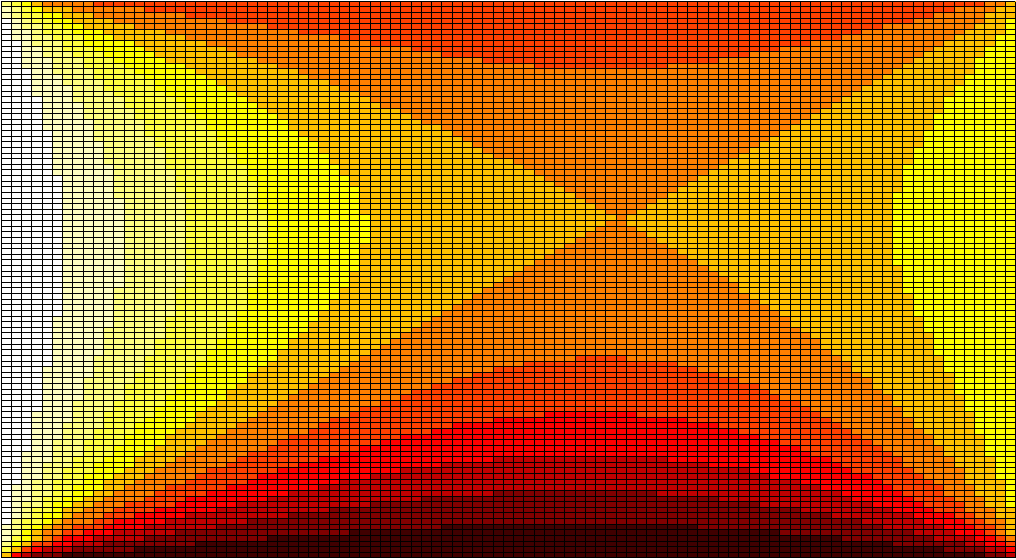
\includegraphics[width=.7\textwidth]{10-20-30-40.png}
\caption{Todos os lados diferentes}
\label{fig:1}
\end{figure}

Na Figura \ref{fig:2} representa o resultado da placa com temperatura acima, abaixo, lateral esquerda e lateral direita, equivalentes a \SI{40}{\celsius}, \SI{10}{\celsius}, \SI{20}{\celsius}, \SI{20}{\celsius} respectivamente. Notemos que o gradiente de cores é uniforme nas laterais por serem de mesma temperatura e se dissipa de baixo para cima, formando um espécie de parábola. São as curvas de transferência de calor.

\begin{figure}[h]
\centering
\includegraphics[width=.7\textwidth]{40-10-20-20.png}
\caption{Dois lados iguais e dois diferentes}
\label{fig:2}
\end{figure}

\section{Conclusão}

A partir dos resultdos obtidos, confirmamos que os gradientes encontrados são os resultado esperado baseado nos outros trabalhos. Logo todos sistemas lineares solucionados para chegar no resultado estão coerentes. Logo temos que foi concluído o objetivo de demonstrar a interação entre a computação e a aplicação matemática desmonstrada neste trabalho, a interação entre a matemática e a computação se torna evidente e essêncial de forma evidente com a realização deste trabalho. A aplicação dos estudos de transferência de calor pode se estender e ficar bem mais complexas. Por enquanto, vamos nos ater so até os resultados obtidos neste trabalho, mas com isso temos uma pequena visão de como a computação, matemática e física estão relacionadas entre si.

\bibliographystyle{sbc}
\bibliography{sbc-template}

%Marcelo A. dos Santos – UFRGS : Novas tecnologias no ensino da matemática, http://www.pucrs.br/ciencias/viali/tic$_$literatura/artigos/tics/101092011085446.pdf

%Waldiney B. , Ismar F. Silveira – UNICSUL : análise e aplicação de software livre parao estudo de construções gráficas na geometria,
%http://www.exatas.ufpr.br/portal/docs$_$degraf/artigos$_$graphica/

%http://www.matematica.pucminas.br/profs/web$_$silvi/calculo2/artigos/show$_$file.pdf

%https://www.mat.uc.pt/~jaimecs/nonius/nonius2$_$1.html

%Álgebra Linear - Jose Luiz Boldrini

%História da computação: O caminho do pensamento e da tecnologia – PUCRS


\end{document}
